This thesis details original experimental investigations in to the interaction of light with the mobile electrons at the surface of metallic diffraction gratings. The resulting quantised surface waves, \textit{surface plasmon polaritons}, have been investigated by optical scientists for over a century, yet interest in the field has never been higher, and progress has never been faster \cite{Barnes2003,Editorial2012}. This is due in large part to the relatively recent advances in nano-fabrication techniques, which have allowed greater control over the surface wave propagation and dispersion characteristics on metallic surfaces. This work endeavours to extend the understanding of surface plasmon polaritons on diffraction gratings by exploring their propagation along symmetries and structures that have not been reported previously, and whose fabrication has only recently become achievable.

\section{History}
The phenomenon of diffraction from gratings has been reported by scientists since Francis Hopkinson peered at a street lamp through a silk handkerchief in 1785 \cite{Rittenhause1786,loewen1997diffraction}. The rainbow that is seen due to the dispersion of light through such fine structure was recognised immediately as an incredibly useful optical property by Fraunhofer, and it was not long before early diffraction gratings were being manufactured by scratching fine grooves in to the surfaces of glasses and metals.

In 1902, it was these early forays into the structuring of metals that led to the first recorded observations of surface plasmon polaritons' interaction with light. Wood \cite{Light} reported a bright band of enhanced reflection and a dark band of low reflection found in the projected spectrum of a ruled speculum diffraction grating produced at John Hopkins University \cite{Strong1960}. Diffraction gratings produced by these early ruling engines were finding a multitude of uses in physics at the time, particularly in the young field of spectroscopy, and an explanation of Wood's spectral anomalies was vigorously sought. Lord Rayleigh explained the observed dark band in his theory of diffraction gratings in 1907 \cite{Rayleigh1907a} as the wavelength of incident light at which a diffracted light ray will start, or cease, to propagate. The redistribution of available propagating energy at this point created a reflectivity feature corresponding to one of the two Wood's anomalies. Thereafter this was referred to as the `Rayleigh anomaly' \index{Rayleigh} and today this is also called the `diffraction edge' or `pseudo-critical edge'.

Wood's bright band was left unexplained for nearly thirty years until Strong \cite{Strong1936}, attempting to improve the reflective efficiency of a set of gratings by coating them with different types of metals, noticed the band shifted in energy depending on the metal coating used. This dependence on the metal's optical characteristics led Ugo Fano \cite{Fano1936,Fano1941,Fano1937}, to the conclusion that this reflectivity anomaly was a signature of interactions of light with a trapped surface wave, comprised in part by the metal's conduction electrons at the surface. He took the view that this represented a `zero-order' waveguide mode: a guided mode that could still exist localised to the surface when a hypothetical supporting waveguide over-layer was decreased to zero thickness. Maxwell's equations provided Fano with a solution for such a wave, on the condition that one material was a conductor and the other a dielectric\footnote{Unbeknownst to Fano, similar work had been pursued by Zenneck \cite{Zenneck1907a} and also Sommerfeld \cite{Sommerfeld1909} in their research on the transmission of radio-waves across large distances using trapped surface waves between seawater and air.}. Today we call this interface mode a surface plasmon polariton (SPP) and it is defined as an electromagnetic surface wave bound to the interface between a conductor and a dielectric. 

While the first recorded observation of SPPs was on a diffraction grating, SPPs are not unique to these devices alone, and are generally found in systems where a conducting/dielectric interface exists. Once Fano had underpinned the physical origin of this surface wave, and in particular the momentum requirements to resonantly drive it, other methods by which to excite SPP on metal surfaces began to emerge. In the late 1950s, Ritchie \cite{Ritchie1957} and Ferrell \cite{Ferrell1958} both predicted the excitation of SPPs on thin, flat, metal films with accelerated electrons, with Ferrell also predicting the SPPs could decay back into light. This prediction was confirmed experimentally by Steinmann \cite{Steinmann1960} two years later. Today, the use of electrons to excite SPPs has found application as a very precise method of plasmonic investigation: electron energy loss spectroscopy \cite{Abajo2008}. 

In 1968, Otto \cite{Otto1968} and simultaneously Kretschman \& Raether \cite{Kretschmann1968} excited SPPs using a prism geometry\footnote{Turbadar \cite{Turbadar1959} was the first to excite this wave using a prism geometry, but unfortunately failed to connect his work to that of Fano or his observed phenomena to SPPs.}. This technique used the evanescent `tail' of light undergoing total internal reflection in the prism to couple to SPPs on a metal/air interface, matching the momentum of the SPP field through the classical tunnelling of the evanescent wave originating from inside the high-index material. Their techniques for prism coupling are still used today, particularly in SPP based sensors which can investigate a diverse range of analytes, including the detection of fake tequila \cite{Monzo2011} and other spirits \cite{Mitsushio2012}. 

Research in to SPPs on diffraction gratings continued in parallel with the development of these other excitation methods, with their observation and dispersion being investigated in the 1960s \cite{Stewart1962,Hagglund1966,Ritchie1968}. Research in the 1970s and 1980s focussed on the effect of deep grooves \cite{Inagaki:86,Maradudin1982,Laks1981,Ly1981} and over-layer coatings \cite{Introduction1970,Chandezon1982}, driven in part by the development of holographic methods for diffraction grating manufacture \cite{Palmer2005}. This was followed by work in the 1990s that explained the influence of the grating shape on the resonances \cite{Watts1999}, SPP's role in polarisation conversion \cite{Bryan-Brown1990} and the physical origin of observed SPP band interactions \cite{Barnes1995}. 

With the advances in nano-fabrication techniques, the development of detailed theoretical treatments for diffraction problems \cite{Bao} and the increasing affordability and power of computers, increasingly complex diffraction grating geometries could be explored. The combinations of all these factors also helped spawn the active research field of `plasmonics', and further improvements in all these areas continue to be a driving force behind the latest SPP research. 

SPPs on gratings have already found many applications, and in some cases are already integral to commercial products. With the energy of a SPP resonance being  highly sensitive to the local environment at the surface, SPPs have been used very successfully in sensing applications  \cite{Tu1999,Bog2012,Singh2006}; these have included the in-situ monitoring of chemical reactions such as catalytic conversion \cite{Janssens2007,Lindfors2004},
non-contact determination of surface structure \cite{Watts1998, T.Hallam2000}, and the measurement of optical constants of metals \cite{Watts1996}. 

Coupled SPPs on gratings have also been used to enhance various optoelectronic devices; improvements to photo-detectors \cite{Butun2012}, the enhancement of laser beams \cite{Oulton2009,H'Dhili2011,Okamoto2008,Berini2011}
and the ability to improve the efficiency of solar cells \cite{Polman2012,Ferry2011,VandeGroep2012,VanLare2012,Sha2012}   have all been reported in the literature. Generation of radiation has also been achieved on metallic or semiconducting gratings through SPP mediated second harmonic generation \cite{Zayats2005} or by SPPs stimulating electron photo-emission leading to the production of terahertz scale radiation \cite{Welsh2007, Shubina2011a}. 

Additionally, SPPs on gratings have been employed as optical elements including colour filters \cite{Cheong2009}, polarisation converters \cite{Watts1997a}, and various surface optics for collimation or achieving negative refraction \cite{Yu2010,Stein2012}. They have also been used for the novel demonstration of enhanced transmission through hole arrays \cite{Ebbesen1998,Lezec2002a,Mahboub2010a,Garcia-Vidal2005} and the manipulation of Magneto-optical effects such as Faraday and Kerr rotations \cite{Belotelov2007}. The use of SPPs will no doubt continue to find applications in the most recent of technologies, particularly with very recent demonstration of their excitation on graphene \cite{Chen2012}.

This brief review of the investigations and applications of SPPs on gratings leads us to the present day and the theme of this thesis. In this work, unconventional gratings are used to couple to SPPs, and the propagation and dispersion of SPPs on such gratings is investigated. The experiments presented here are done to explore the properties of SPPs on novel types of grating, and do not attempt to fit any particular application. However, many possibilities for extensions or applications are possible, and these are suggested in each chapter and summarised in the conclusions.


\section{Scope and Outline of This Work}

This thesis details experimental investigations into the propagation of SPPs on diffraction gratings that possess novel structure or symmetries. Broadly it may be divided up in to investigations of two types of diffraction grating; `crossed' bigratings and a new type of diffractive optical element: the `zigzag grating'. Since both these types of grating possess two different diffractive periods in their surface geometry, they may both be considered a type of the larger family of metallic `bigratings'. There are four diffraction grating geometries investigated in this work, and these are summarised in figure \ref{fig:intro-thegratings}. They are; the rectangular bigrating, the oblique bigrating, the `zigzag grating' and the `asymmetric zigzag grating'.

\begin{figure}
\begin{center}
\subfigure[Rectangular]{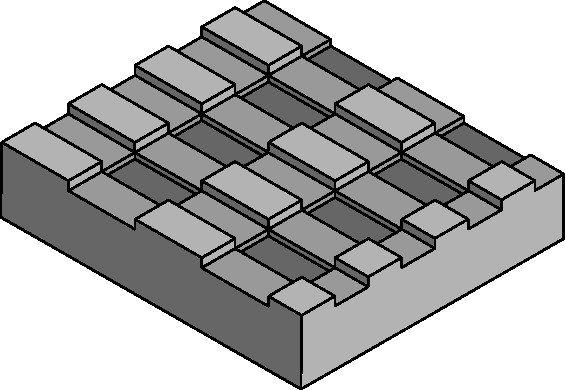
\includegraphics[width=0.33\linewidth]{figure-rect.pdf}}
\subfigure[Oblique]{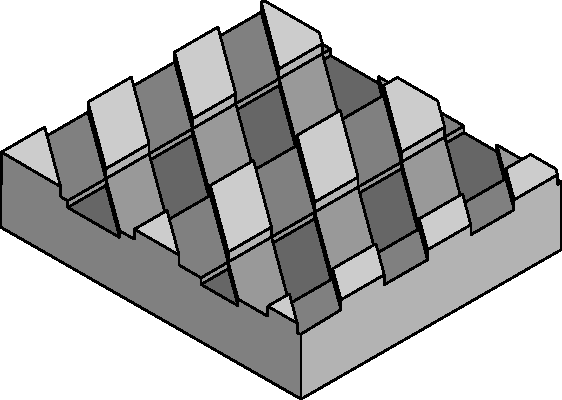
\includegraphics[width=0.33\linewidth]{figure-oblique.pdf}}\\
\subfigure[Symmetric Zigzag]{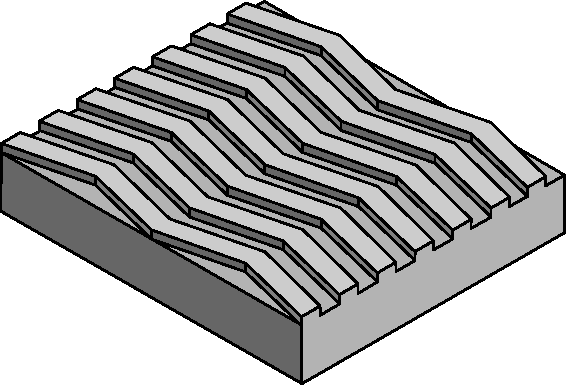
\includegraphics[width=0.33\linewidth]{figure-zigzag.pdf}}
\subfigure[Asymmetric Zigzag]{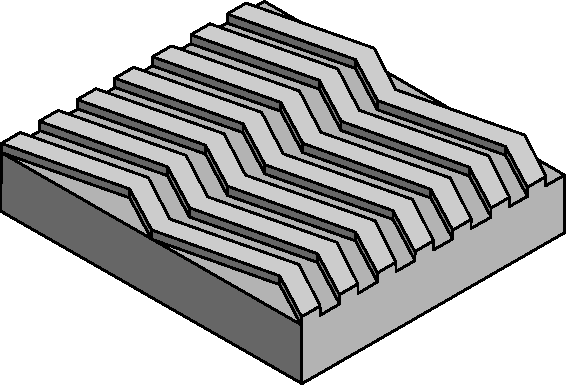
\includegraphics[width=0.33\linewidth]{figure-asymmetric-zigzag.pdf}}
\end{center}
\caption[The four types of grating geometry that are investigated in this thesis: The rectangular bigrating, the oblique bigrating, the zigzag grating, and the asymmetric zigzag grating.]{The four types of grating geometry that are investigated in this thesis: (a) The rectangular bigrating in chapter \ref{c:rectangular}, (b) the oblique bigrating in chapter \ref{c:oblique}, (c) the zigzag grating in chapter \ref{c:zigzag} and (d) the asymmetric zigzag grating in chapter \ref{c:azigzag}. \label{fig:intro-thegratings}}
\end{figure}

The background theory of SPPs on both planar films and on metallic diffraction gratings is presented in chapter \ref{c:backgroundtheory}. This chapter covers the origin, coupling conditions and band-structure of SPPs on both planar and periodic surfaces. The methods by which the optical response of the gratings under consideration have been calculated theoretically are then explained in chapter \ref{c:theorymethods}.

Chapter \ref{c:experimentalmethods} details the experimental methods used for the production and measurements of gratings in this thesis. In addition to the standard experimental techniques used, a new method by which to map the plasmonic analogue to the iso-frequency `Fermi-contours' of the SPP band structure is presented. These iso-frequency contours have been recorded using imaging scatterometry and this new technique, developed as part of this body of work, is used extensively throughout this thesis.

Chapter \ref{c:rectangular} presents some experimental observations on the excited SPPs supported by rectangular bigratings. These are gratings formed of two diffraction gratings of different pitch, crossed relative to each other at an angle of $90^\circ$. The dispersion of these modes on the surface and the formation of standing surface-wave states are experimentally recorded and matched to a theoretical model. It is found that by deepening the grooves of one of the constituent diffraction gratings, the propagation of SPPs along the surface becomes highly anisotropic. Control over this effective mode index in different directions along the surface  could find application in surface-wave optics devices.

The work on `crossed' bigratings continues in chapter \ref{c:oblique}, with the experimental investigation of SPPs on a bigrating with the reduced symmetry of an oblique lattice. The dispersion and scattering mechanisms on a fabricated oblique grating are recorded experimentally and explained. SPP mediated polarisation conversion is also observed on these gratings, as the scattered surface fields propagate along a surface of no mirror symmetry. The lack of symmetry on such a grating leads to the observation of SPP band gaps not forming at the Brillioun Zone (BZ) boundaries, and a general discussion of the oblique symmetry constraints on SPPs is offered to explain why this is so.

Chapter \ref{c:zigzag} introduces a new type of diffraction grating, the `zigzag grating'. This grating uses sub-wavelength structure in one direction to introduce an diffractive periodicity in the orthogonal direction. It is found, experientially and theoretically, that even-order diffracted fields only couple to SPPs for one linear polarisation of light, while odd-order diffracted fields only couple to the other, orthogonally polarised light. Further, it is shown that SPP band gaps are forbidden at the first BZ boundary by the symmetry of the zigzag surface. Finally in this chapter, it is shown that the sub-wavelength grooves on such a grating can lead to highly anisotropic SPP propagation. This anisotropy leads to SPP propagation at certain frequencies in only one single direction, irrespective of excitation angle. When combined with the lack of band gaps on such a symmetry, this makes these gratings excellent candidates for surface wave collimation devices.

The final experimental results of the thesis are presented in chapter \ref{c:azigzag}, which extends the zigzag grating geometry to one with reduced symmetry. This relaxes the polarisation conditions of the previous zigzag grating, leading to \textit{any} SPP being coupled to with \textit{any} incident polarisation of light, a result which could prove relevant to improving the efficiency of many plasmonic devices. The band structure of the SPPs supported by this grating is also experimentally investigated and the coupling to the different standing wave states by light which occur at the first BZ boundary is explored. The SPP anisotropy previously found for a zigzag grating is also found in this new asymmetric zigzag grating case, and combined with the large band gaps which form at the first BZ boundary, the grating is shown to support a full plasmonic band gap, for which SPP propagation is forbidden in all directions.

The thesis is concluded in chapter \ref{c:conclusions} with a summary of the findings and suggested future research which could extend the findings and applications of this work.





